\documentclass[%
12pt,
master,         % тип документа
natbib,         % использовать пакет natbib для "сжатия" цитирований
subf,           % использовать пакет subcaption для вложенной нумерации рисунков
href,           % использовать пакет hyperref для создания гиперссылок
colorlinks=true % цветные гиперссылки
%,fixint=false  % отключить прямые знаки интегралов
%,times         % шрифт Times как основной
]{disser}

% Original: left - 2.5, right - 1, baseline untouched
\renewcommand{\baselinestretch}{1.5}
\usepackage[
  a4paper, mag=1000,
  left=3cm, right=2cm, top=2cm, bottom=2cm, headsep=0.7cm, footskip=1cm
]{geometry}
\usepackage[T2A]{fontenc}
\usepackage[utf8]{inputenc}
\usepackage[english,russian]{babel}
%\usepackage{tabularx,longtable}
\ifpdf\usepackage{epstopdf}\fi
% Номера страниц снизу и по центру
%\pagestyle{footcenter}
%\chapterpagestyle{footcenter}

\usepackage{xcolor}
\usepackage{listings}
\lstset{basicstyle=\ttfamily,
  showstringspaces=false,
%  commentstyle=\color{red},
%  keywordstyle=\color{blue}
}

% Точка с запятой в качестве разделителя между номерами цитирований
%\setcitestyle{semicolon}

% Использовать полужирное начертание для векторов
\let\vec=\mathbf

% Включать подсекции в оглавление
\setcounter{tocdepth}{2}

\graphicspath{{fig/}}

\begin{document}

% Переопределение стандартных заголовков
%\def\contentsname{Содержание}
%\def\conclusionname{Выводы}
%\def\bibname{Литература}

\institution{Министерство образования и науки Российской Федерации\\
			Московский физико-технический институт {\rm(государственный университет)}\\
			Факультет управления и прикладной математики\\
			Кафедра информатики}

% Имя лица, допускающего к защите (зав. кафедрой)
\apname{Петров Игорь Борисович}

\title{ДИССЕРТАЦИЯ\\[-14pt]на соискание ученой степени\\МАГИСТРА}

\topic{Разработка модели среды распределенных вычислений Evergrid для сравнения алгоритмов управления потоками задач и данных}

% Автор
\author       {Колеснев Роман Владимирович} % ФИО
\group        {073а} % Группа
\coursenum    {03.04.01} % Номер направления
\course       {Прикладные математика и физика}
\masterprognum{010956} % Номер магистерской программы
\masterprog   {Математические и информационные технологии}

% Научный руководитель
\sa      {Устюжанин Андрей Евгеньевич}
\sastatus{к.~ф.-м.~н., доцент}

% Рецензент
\rev      {Рыков Владимир Васильевич}
\revstatus{к.~л.~н., доцент}

% Город и год
\city{Москва}
\date{\number2016}

\maketitle

\tableofcontents
\intro

\chapter{Название главы}


\chapter{Постановка решаемых в дипломе задач}

\textit{evergrid - большой проект и в рамках одной дипломной работы его не сделать.}

\textit{Краткое перечисление решаемых задач: сформулировать архитектуру, сделать первичный выбор технологий, построить среду моделирования для проверок гипотез об алгоритмах}

\textit{Архитектура. Глобальное видение должно быть сразу, пусть оно и имеет риск к изменениям. Архитектура специфична. Не стоит спускаться до мелочей, но глобально все должно быть расписано сейчас.}

\textit{Выбор технологий, языков и инструментов важен по различным причинам}

\textit{Среда моделирования позволяет "прочувствовать" как работает архитектура на ранних этапах, недостаток решений в этом сегменте, интероперабельность повысит стабильность продукта.}

\textit{Необходимость нескольких "проверочных" алгоритмов.}
\chapter{Спроектированная архитектура}

\section{Основные ограничения}

Проектирование хорошей архитектуры основывается на:

\begin{itemize}
	\item достаточно подробной постановке задачи
	\item выявлении ограничений
	\item использовании актуальных технологий как составных блоков
	\item максимальной простоте реализации не в ущерб необходимому уровню качества
\end{itemize}

Постановка задачи у нас есть, последние два пункта постараемся соблюдать. Осталось понять, какие у нас ограничения. Под ограничениями понимаются технические аспекты, которые напрямую следуют из постановки задачи и ограничивают нас в свободе выбора тех или иных технологий, тех или иных подходов. В этом разделе я приведу те ограничения, которые считаются неочевидными или заслуживающими отдельного упоминания.

Первое из них - связанное с безопасностью. Мы используем вычислительные ресурсы, предоставляемые третьими лицами. И они имеют неограниченный (root) доступ к ним. Поскольку процесс предоставления этих ресурсов подразумевается достаточно свободным, будет правильно представить злоумышленника на месте поставщика мощностей. Какие потенциальные угрозы он может предоставлять?

\begin{itemize}
	\item захват не принадлежащих ему ресурсов
	\item нарушение работы кластера (например, вмешательство в работу планировщика)
	\item нарушение корректной работы предоставленного вычислительного ресурса (фальсификация результатов, намеренное замедление скорости вычислений и т. п.)
\end{itemize}

Первые две угрозы нивелируются достаточно просто: \textit{на арендуемых ресурсах не должен выполняться код, связанный с управлением кластером. Только выполнение задач и отправка результатов.}

Третья - наиболее сложная. Но риски можно свести к минимуму, если \textit{вообще не запускать на арендуемых ресурсах компоненты системы}. Естественной реализацией этого принципа является удаленное управление по SSH. Тогда злоумышленник будет знать минимум о текущем состоянии системы. Прочие методы борьбы с этой угрозой уже выходят за рамки этой работы.

Следующее ограничение происходит из того, как мы будем выполнять задачи. Очевидно, что нам нужна виртуализация - иначе наш кластер быстро превратят в ботнет. Нам нужна универсальность - хочется покрыть как можно больше сценариев использования. Также нам нужна скорость - следовательно, нам нужна легковесная виртуализация. Третий критерий - технология должна быть простой в использовании. В идеале - проведение эксперимента на своей локальной машине не должно отличаться от выполнения его на наших мощностях. Сложив все эти требования воедино, мы получим ответ - Docker. И это решение имеет много преимуществ: Docker отлично отвечает требованиям к изоляции, удобству воспроизводимости и модификации. А его инструментарий органично вписывается в архитектуру. От предоставляемых мощностей нам в итоге требуется:

\begin{itemize}
	\item свободное место на диске
	\item доступ по ssh
	\item корректно работающий docker
	\item возможность мониторинга нагрузки (чтобы регистрировать не относящуюся к нашему сервису нагрузку)
\end{itemize}

Даже неограниченный доступ в Интернет не является жестким требованием - мы можем собрать контейнер на наших машинах и готовый образ передать по ssh.

Возникает вопрос о том, как пользователь должен предоставлять контейнер со своим алгоритмом. Если следовать идеям доступности и простоты модификации, то наиболее очевидное решение - Github. Наиболее органично будет работать с специально оформленными github-репозиториями, которые содержат все необходимое для сборки контейнера.

Использование Docker на первый взгляд накладывает ограничение вида ,,одна задача = одна машина'', но это можно обойти - ведь мы можем активизировать несколько машин и разрешить контейнерам общаться между собой. Тем не менее, в рамках данной работы акцент сделан именно на подходе "одна задача = одна машина". Несмотря на это, архитектура должна быть пригодна для обоих вариантов.

Если уж рассмотрели то, как загружать реализации алгоритмов (далее будем называть их контейнерами, раз имеем в виду Docker) - то стоит сказать пару слов о загрузке датасетов. Никаких особых ограничений здесь незаметно. Все, что нужно - это иметь системе возможность закачать собранный контейнер на свои машины. Путей достижения этого много, и в данной работе они не будут рассматриваться (за исключением перемещения датасетов внутри самой системы).

И последнее ограничение, о котором я хочу сказать, - это CAP-теорема. Мы имеем дело с распределенной в глобальной сети системой, а в таком случае нельзя забывать о CAP-теореме. Нарушение связи между элементами системы не должно приводить к ее некорректной работе.

\pagebreak

\section{Предлагаемая архитектура}

\begin{figure}
	\centering
	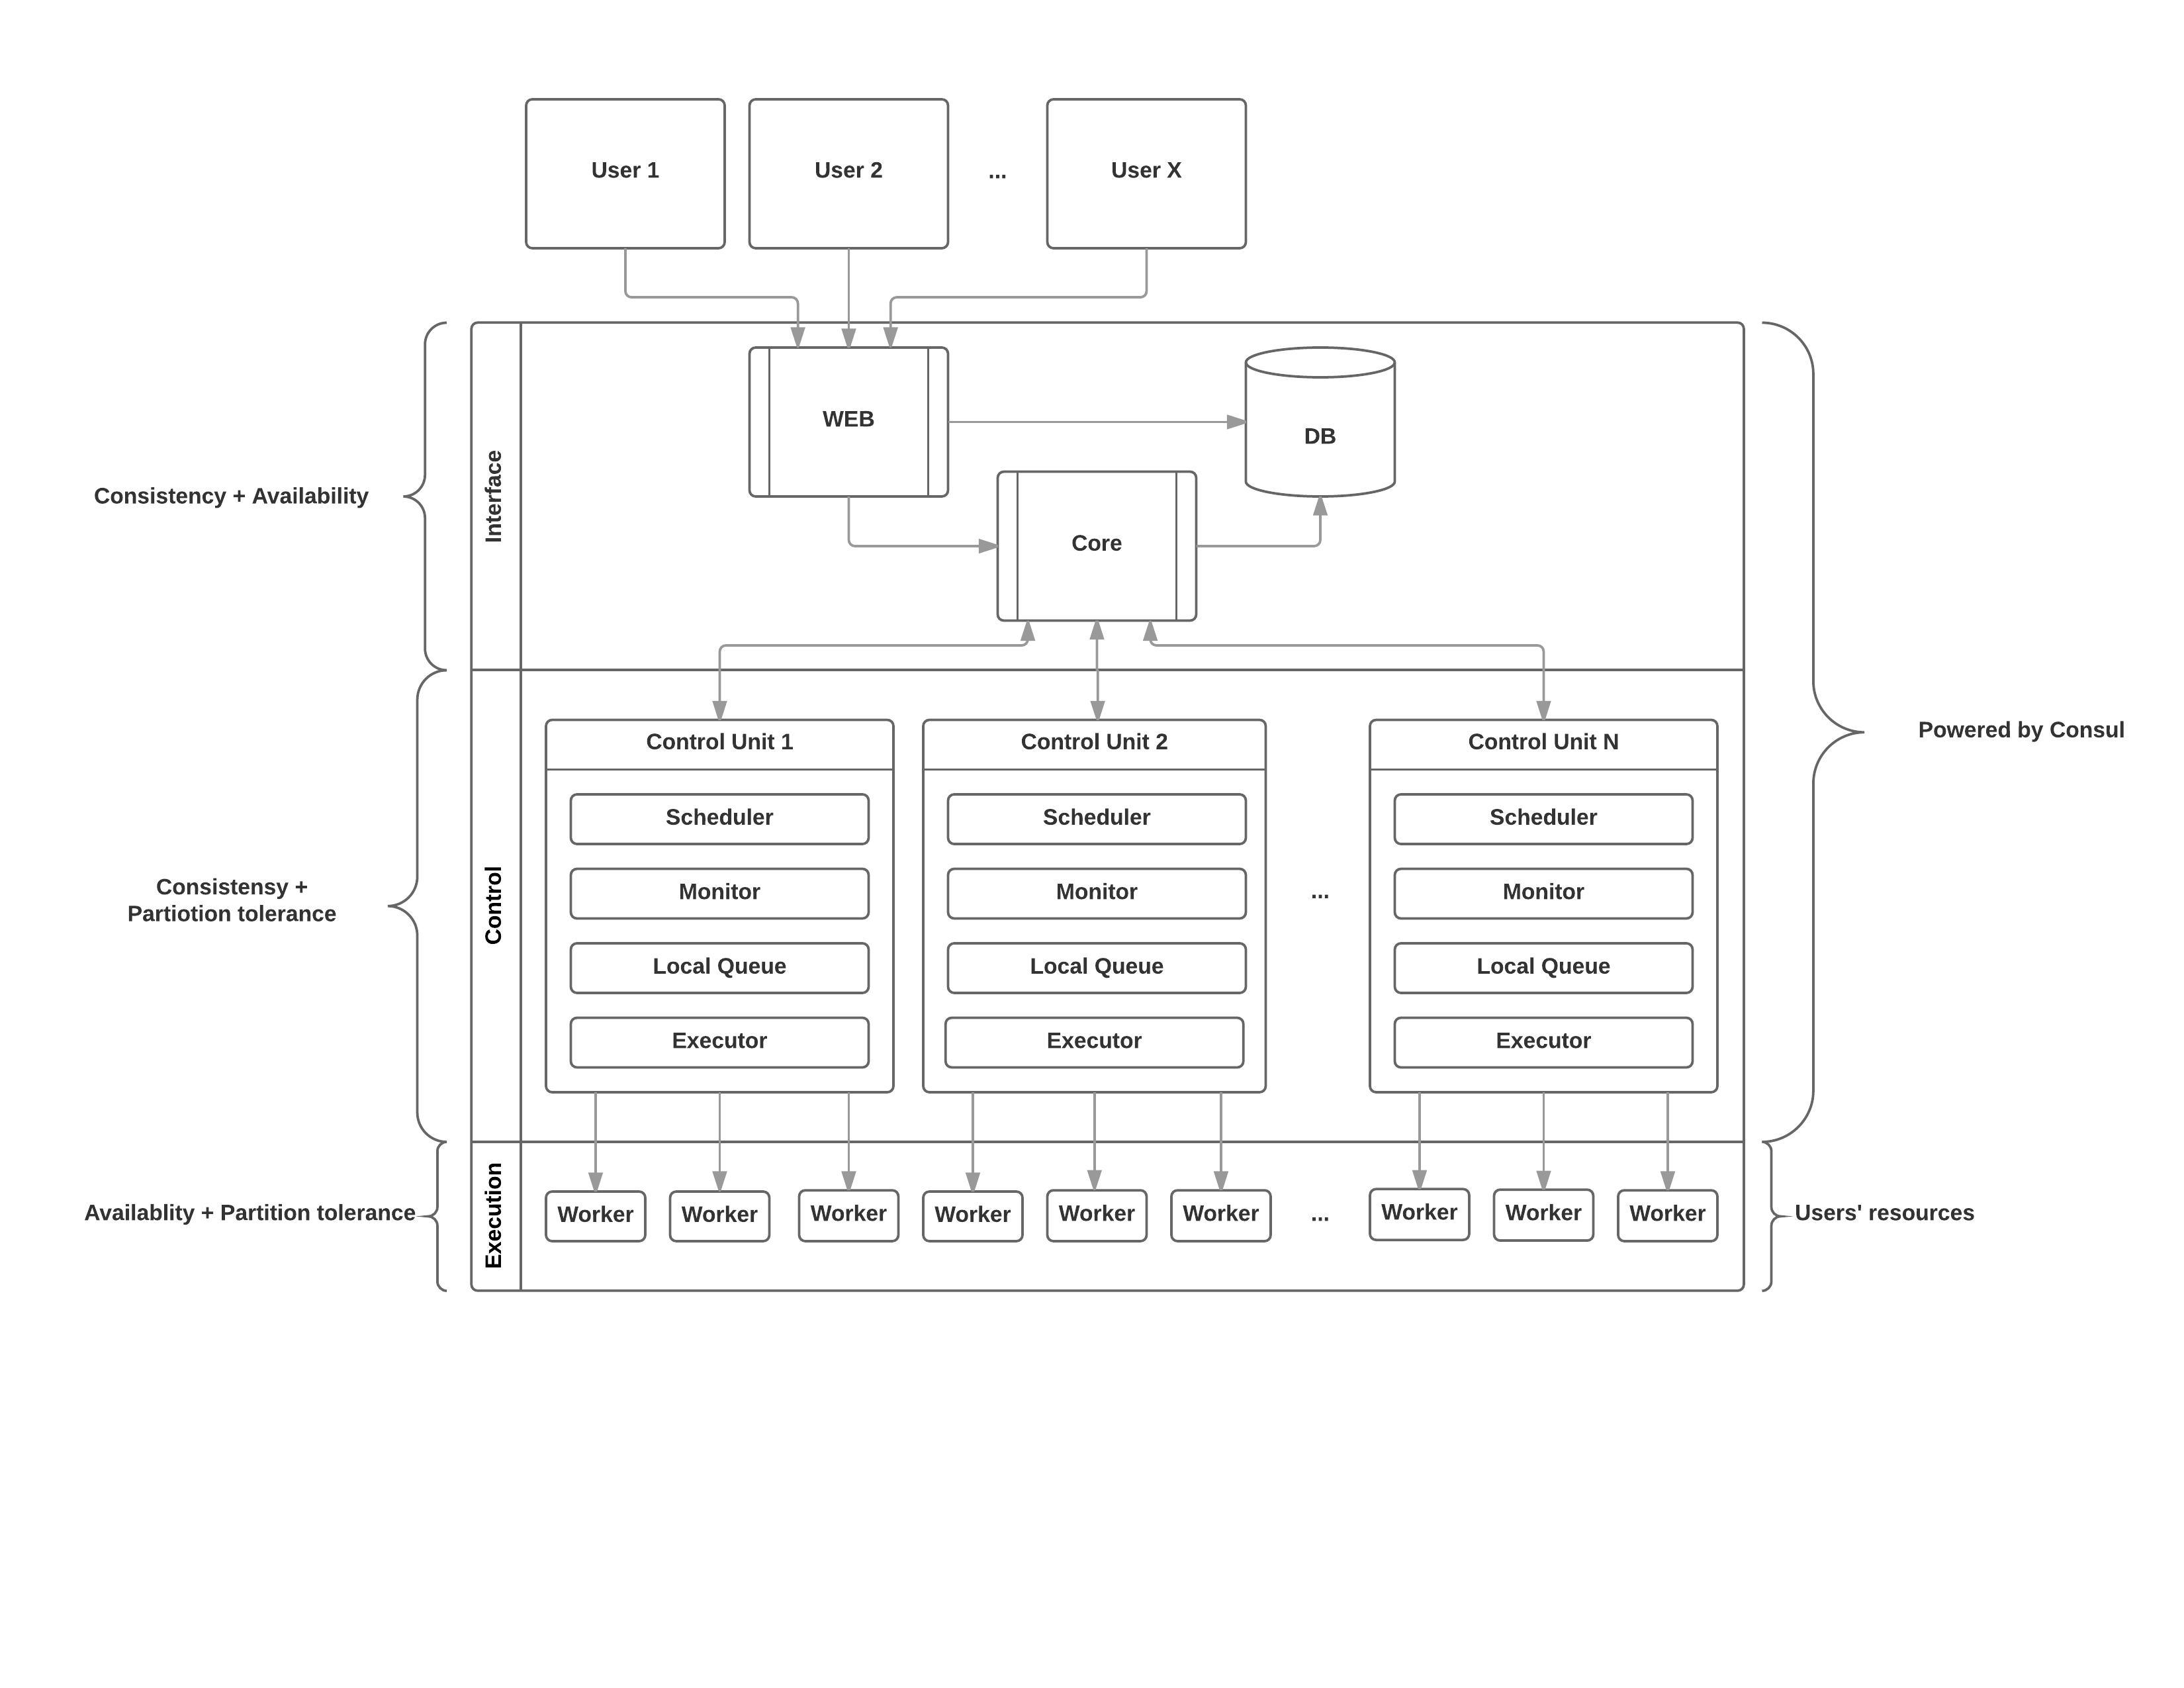
\includegraphics[width=\textwidth]{fig/architecture}
	\caption{Диаграмма архитектуры}\label{fig:architecture}
\end{figure}

Теперь можно рассмотреть конкретную реализацию, удовлетворяющую описанным выше принципам. Диаграмма предлагаемой архитектуры показана на рисунке \ref{fig:architecture}. Далее мы рассмотрим в отдельности каждый из ее слоев и компонентов.

Для начала объясню общую структуру. Здесь видно разделение на три слоя плюс пользователи системы. User 1 -- User X - это пользователи. Каждый слой состоит из компонентов. Распределение компонентов по машинам специфично для каждого слоя. Для слоя Interface оно явно не ограничивается предложенной архитектурой. В зависимости от нагрузки и прочих факторов все эти компоненты могут быть как на одной машине, так и разнесены по нескольким. Для слоя Control истинно правило "одна машина - один Control Unit". Для слоя Execution все просто - один Worker равен одной машине, предоставленной для вычислений.

Направление стрелок - это направление запросов между компонентами. В случае долговременного соединения - стрелка направлена от инициатора.

Первые два слоя - это “наши” машины, которым мы доверяем, и только у нас есть к ним доступ.

Третий слой - машины, предоставленные извне, мы им “не доверяем”.

Слева показаны приоритеты в терминах CAP-теоремы для каждого слоя.

Справа показано, что первые два слоя используют Hashicorp Consul для service discovery и leader election.

\subsection{Слой Execution}

На этом слое находятся машины, предоставленные пользователями системы. Они частично конфигурируются нами и не содержат никакого кода, который бы управлял слоями выше (из соображений безопасности). Про специфику работы с этими ресурсами и требования к ним было написано выше.

Все запросы приходят со слоя Control. То есть машинам даже необязательно знать IP других компонентов системы. Отдельный случай - если машины не имеют ''белого'' IP: в этом случае в их обязанность входит самостоятельно поддерживать соединение со слоем Control, и нам все же придется ставить на Worker'ы какое-нибудь приложение, которое будет обеспечивать соединение со слоем Core.

\subsection{Слой Control}

Состоит только из Control Unit’ов. Каждый Control Unit - это отдельная машина. Каждый Worker из слоя ниже принадлежит только одному Сontrol Unit’y.

Control Unit состоит из нескольких логических компонент и представляет из себя монолитную программу.

Все Control Unit с этого слоя представляют из себя распределенную систему. То есть запросы с верхнего слоя Interface по своей сути направлены не к конкретному Control Unit'у, а ко всей системе целиком.

Смысл подобного разбиения - это большая стабильность системы. Т. е. эффективным подходом будет, например, расположить по одному Control Unit на географическую зону.

Смысл всей этой системы в следующем:

\begin{itemize}
	\item Получать задания со слоя выше (от Сore)
	\item Раскидывать датасеты по Worker’ам
	\item Запускать вычисления на Worker’ах
	\item Отправлять результаты вычислений на Worker’ах на слой выше (в Core).
\end{itemize}

Теперь конкретные примеры запросов, которые могут приходить в эту систему:

\begin{itemize}
	\item Загрузи датасет
	\item Загрузи и собери этот docker-контейнер
	\item Обнови этот докер контейнер
	\item Обнови этот датасет
	\item Запусти этот контейнер с этим датасетом
\end{itemize}

Из подобных задач формируются локальные очереди (Local Queue). В какую локальную очередь и на какой Worker отправить задачу, определяет “распределенный” Scheduler. Также состояние, корректность и доступность Worker'ов, прочие глобальные характеристики системы отслеживаются Monitor'ом. Monitor может давать информацию о всех доступных Worker'ах системы. Monitor - основной инструмент Scheduler'а для получения текущего состояния системы. Executor отвечает за "опустошение" очереди и выполнение задач на Worker'ах.

Результат выполнения работы отправляется в Core, который, в свою очередь, решает, где хранить этот результат.

\subsection{Слой Interface}

Распределение по машинам в этом слое диктуется лишь нагрузкой. При малом количестве пользователей - можно все три компонента держать на одной машине. Теперь отдельно про каждый компонент.

\begin{description}
  \item[WEB] Веб-приложение, написанное на любом адекватном web-фреймворке. Именно через него происходит постановка задач, просмотр результатов и прочее. Является единой точкой управления системой как для рядовых пользователей, так и для администраторов. Важно понимать, что здесь используются не только HTML + JS, но и реализована вся бизнес-логика интерфейса.
  \item[DB] Основная база данных. В ней хранится все относящееся к бизнес-логике приложения. По своему содержанию должна быть независима от нижестоящих слоев. Т. е. если конфигурация всего того, что есть ниже, станет иной - данные не должны стать некорректными.
  \item[Core] WEB не общается напрямую со слоем Сontrol. Он работает с Core через API, а оно в свою очередь контролирует слой ниже. Т. е. Core - это микросервис взаимодействия со слоем Control. Это важное разделение, поэтому подчеркну: WEB - это бизнес логика, Core - микросервис, который контролирует общение с распределенной вычислительной системой. Core не проверяет никаких параметров, связанных с бизнес-логикой: кто поставил задачу, сколько у него денег на счету и прочее. 
\end{description}

\section{Выбор технологий для реализаций компонентов}

Теперь, когда есть представление о структуре, надо понять, какие есть эффективные способы реализации. Если не оговорено иного, предложенные способы несут рекомендательный характер.

\subsection{WEB}

Посколько Evergrid является по своей сути стартапом, то важным аспектом является скорость разработки. То есть надо уметь быстро создать прототип и иметь возможно быстро вносить изменения. На Java и ASP.NET подобное получается плохо, особенно у небольших команд. Наиболее успешно используемые технологии - это Ruby on Rails\footnote{\url{http://rubyonrails.org/}} , Node.js\footnote{\url{https://nodejs.org/en/}} фреймворки\footnote{Например: \url{http://expressjs.com/}} , Django\footnote{\url{https://www.djangoproject.com/}} и прочие python-фреймворки, PHP\footnote{\url{http://php.net/}}.

Есть также менее распространенные решения, но тоже заслуживающие внимания: Play Framework\footnote{\url{https://www.playframework.com/}} , Phoenix Framework\footnote{\url{http://www.phoenixframework.org/}}.

Веб-фреймворки можно разделить на два класса:

\begin{description}
  \item[С "синхронной" архитектурой] -- когда запускается ровно N обработчиков запросов (в отдельных процессах или тредах). То есть система может одновременно обрабатывать не более чем N запросов. Выполнение запросов изолировано друг от друга. В данных ограничениях удобно писать код, но страдает масштабируемость и не стоит использовать продолжительные по времени подключения (websocket'ы, например). Синхронным такой подход называется т. к. в случае одного обработчика мы блокируем выполнение следующего запроса до завершения предыдущего.
  \item[С "асинхронной" архитектурой] -- в этом подходе для каждого входящего запроса на лету создается свой поток обработки. Т. е. мы, в отличие от предыдущего подхода, не вынуждены ждать завершения обработки предыдущего запроса для начала обработки нового. Для такой архитектуры сложнее писать код, но обычно решения на ней обладают лучшей производительностью и более широким спектром возможностей.
  \item
\end{description}

Это описание, достаточное для общего понимания. Еще один важный параметр - это используемый язык программирования. От него зависит как скорость продукта, так и, отчасти, легкость его сопровождения.

Сначала рассмотрим технологии, использование которых может оказаться неэффективным:

\begin{description}
	\item[Java/ASP.NET] Плохо годятся для небольших команд. ASP.NET плох своим акцентам на Windows-сервера. Java, на фоне прочих языков, слишком "многословна", и быстро реализовать на ней прототип довольно тяжело.
	\item[Node.js] Несмотря на асинхронность архитектуры, javasript работает в одном потоке. Но главный его недостаток - это дизайн языка. У JS крайне слабая система типов, запутанная спецификация и много неоправданно неочевидных моментов.
	\item[PHP] Очень популярен в вебе, до сих пор развивается, множество фреймворков. Но дизайн языка хоть и лучше, чем у JS, все равно уступает ruby и python. Другой его недостаток - слабость как языка общего назначения - выражается в том, что на нем неудобно писать что-то кроме непосредственно генерации ответов на запросы к веб-серверу. А подобное может понадобиться - например, для организации выполнения внешних очередей задач или удобного использования websocket'ов. Кратко говоря, PHP неоправданно накладывает слишком много ограничений.
\end{description}

Теперь рассмотрим список технологий, хорошо подходящих этому проекту:

\begin{description}
	\item[Python] Python активно используется как для веб-разработки, так и для научных целей. Веб-фреймворки на нем довольно качественные, и есть большое количество решений для типовых задач (например, регистрация пользователей и пр.). Поскольку Python скриптовый язык с GIL, большинство решений на нем реализуют синхронную архитектуру. Это не настолько большой недостаток, как может показаться, но, если высокая производительность или использование websocket'ов является критичным, - python может оказаться не лучшим выбором.
	\item[Ruby on Rails] В основном ситуация, схожая с python за исключением следующих различий: редко используется в научной среде; язык более гибкий, но и более сложный, чем python; большее количество библиотек с готовыми решениями для веб-разработки. Отдельным преимуществом является и то, что Rails однозначный лидер среди Ruby-фреймворков, а это означает, что почти любая развитая библиотека умеет корректно с ним работать. В случае с python все более разобщено. То есть, если есть возможность эффективно использовать Rails - то это является удачным решением в рамках синхронной архитектуры.
	\item[Phoenix Framework (Elixir)] Если важно использование асинхронной архитектуры, то стоит вспомнить об Erlang. Продукты, написанные на Erlang, в виду особенностей BEAM (Bogdan/Björn’s Erlang Abstract Machine) и принципов OTP (Open Telecom Platform) отличаются высокой стабильностью и производительностью. Elixir - это молодой язык для BEAM, который более удобен в использовании, имеет больше возможностей, чем Erlang, и может без ограничений использовать его библиотеки. На этом языке реализован Phoenix Framework. Что язык, что сам фреймворк - еще молодые, используются в production, но пока еще не получили широкого распространения. Сам фреймворк удобен в использовании. Данный вариант хорош, если хочется получить преимущества Erlang/OTP-экосистемы: высокая стабильность, высокая производительность на IO задачах, дешевый и удобный параллелизм благодаря green threads и акторной модели, преимущества подходов из функциональной парадигмы программирования.
	\item[Play Framework (Scala)] Еще одно возможное решение, если нужна асинхронность и производительность. Scala - преимущественно функциональный язык программирования поверх JVM, имеющий возможности интероперабельности с Java. Тоже использует акторную модель (Akka). Более зрелое решение, чем phoenix, и более широко распространено на данный момент. Из недостатков можно отметить то, что в Erlang более развитые средства для мониторинга и более стабильная реализация акторной модели и супервизоров. Также Scala является более сложным в изучении и использовании языком, нежели Elixir/Erlang. Из преимуществ можно отметить, что мы получаем доступ к внушительному парку Scala и Java библиотек.
\end{description}


\subsection{Core и Control Unit}

Эти два компонента формируют внутреннюю инфраструктуру сервиса. В данном случае корректным будет следующий список требований:

\begin{itemize}
	\item высокая производительность (система должна адекватно вести себя под высокими нагрузками)
	\item выбранное решение должно использоваться для схожих известных продуктов
	\item иметь развитые библиотеки для сетевого взаимодействия
	\item чем проще будет инициализировать новые сервера - тем лучше
	\item язык должен быть популярен и иметь активное сообщество
	\item простота языка будет плюсом
\end{itemize}

Требование высокой производительности ставит под сомнение использование интерпретируемых языков. Из "быстрых" языков в первую очередь приходят на ум C/C++ и go. ASP.NET плохо дружит с Linux, а Java/Scala довольно прожорливы в плане памяти и не являются простыми в использовании языками. С++ - тоже довольно сложный в использовании язык. Если же внимательнее посмотреть на go, то становится видно, что он является хорошим решением:

\begin{itemize}
	\item на нем написаны продукты hashicorp (nomad, consul), на нем написан docker
	\item скорость выполнения сравнима с C/C++
	\item прост в изучении: опытный программист может освоить все основные возможности языка за пару вечеров
	\item популярен для написания микросервисов
	\item встроенная в язык модель параллелизма CSP
	\item активное сообщество и большое количество готовых библиотек
	\item скомпилированное приложение для своей работы не требует установки самого go или каких-либо специфических пакетов
\end{itemize}

Поэтому для Core и Control Unit go является подходящим выбором. Причем данный выбор имеет жесткий характер, так как симулятор тоже написан на go, и часть его преимуществ основывается на том, что для реализации инфраструктуры тоже будет использоваться этот язык.

\subsection{DB}

На самом деле на данном этапе сложно предсказать все те требования, которые могут возникнуть для основного хранилища. Возможно, даже одного продукта не хватит, и будет использоваться некая комбинация (например: часто можно встретить связки Postgres + Redis).

Но, в качестве решения по умолчанию, стоит рассматривать именно Postgres. На данный момент это наиболее универсальное и активно используемое решение среди open source баз данных.

\section{Ограничения, связанные с CAP-теоремой}

Поскольку мы имеем дело с распределенной системой, то стоит явно указать приоритеты в терминах CAP-теоремы. Причем эти приоритеты отдельные для каждого слоя (именно из-за этого вообще появилось разделение на слои).

Также первый и второй слой используют consul - он предоставляет service discovery и leader election интерфейсы, к тому же он создан для решения этих задач как раз-таки в распределенных системах.


\begin{description}
  \item[Слой Execution] Для этого слоя подходит конфигурация [C]AP. Если машина потеряла связь с системой -- перераспределяем нагрузку. Здесь важно в любой момент времени максимально использовать доступные ресурсы.
  \item[Слой Control] При критичной сегментации сети в слое, Control Unit'ы перестают принимать запросы, но продолжают выполнение локальных очередей. Примерно так выглядит жертва availability во имя consistency и partition tolerance. Стоит сказать, что это довольно грубый подход. Но начать разработку проще именно с него. Как второй шаг может подойти weak consistency подход ("согласованность в итоге").
  \item[Слой Interface] На этом слое крайне важна согласованность данных, а без доступности он не имеет смысла. Поэтому жертвуем partition tolerance.
\end{description}

\section{Требования к симулятору}

Имея описание архитектуры, можно сформулировать список требований к симулятору.

Первое из них связано с симуляцией сети. Для симуляции данной архитектуры нам не важен пинг между ее компонентами. Нам важна только скорость передачи данных между ними и сам факт наличия связи. Отдельный случай - это черезмерно большой пинг - это может повлиять на порядок запросов и подобное. Но по факту нам нужно симулировать не пинг, а факт поздней доставки сообщений. В итоге имеем следующие требования:

\begin{itemize}
	\item симуляция видимости между машинами
	\item симуляция скорости передачи данных
	\item симуляция разрыва соединения
	\item симуляция поздно пришедших сообщений
\end{itemize}

Второе ограничение связанно с тем, что мы должны симулировать время. Т. к. нам важно понимать когда выполнялась задача и сколько времени она выполнялась. Наиболее гибким простым решением является "дискретная" природа симулируемого времени. То есть мы используем дискретный таймер, и каждый агент системы делает ту работу, которую теоретически может успеть за эту дискретную единицу времени.

И третье ограничение - симулятор должен быть достаточно гибким, чтобы при изменении принципов работы компонент можно было легко внести изменения в модель.

Всякий симулятор преследует цель проверки гипотез. В данном случае симулятор должен помогать в исследовании:

\begin{itemize}
	\item эффективности алгоритмов планировщиков
	\item принципов взаимодействия компонентов системы
\end{itemize}
\chapter{Требования к среде моделирования}

\textit{Общая постановка проблемы. Ради чего мы моделируем. Что именно мы моделируем. Жесткие и мягкие требования. Упомянуть, что не все аспекты будут реализованы на первом этапе.}

\textit{Чем мы можем пренебречь и почему. В конце вывести в виде конкретного списка.}

\textit{Чем мы не можем пренебречь и почему. В конце вывести в виде конкретного списка.}

\textit{Пара слов о том, что получилось. Вывести суммарный список требований.}
\chapter{Анализ возможных реализаций}

\textit{На основе списка требований мы ищем. Обрисовать два возможных пути: использовать или адаптировать готовое решение, написать свое (на чем). Начнем с первого.}

\textit{Заранее обрисовать преимущества свого решения: интероперабельность.}

\textit{Рассмотреть simgrid, gridsim, alea и мб еще кого. Доказать для каждого неэффективность использования этого подхода.}

\textit{Рассмотреть вариант собственной реализации. Более глубоко рассмотреть преимущества интероперабельности. Выбор языка очевиден - тот же, что и для основной системы.}

\textit{Подробнее описать, как предложенные ограничения соотносятся с реализацией.}
\chapter{Результаты}

Результатами работы является описание архитектуры (приведенное в тексте диплома) и реализация симулятора доступная на github: \url{https://github.com/ffloyd/evergrid-go}.

Код симулятора продокументирован для облегчения его последующей разработки и модификации. Технические тонкости реализации и более подробное рассмотрение принципов работы отдельных компонентов вынесены за рамки текста диплома и являются частью документации.

Удобная он-лайн версия документации доступна по адресу: \url{https://godoc.org/github.com/ffloyd/evergrid-go}.

Помимо описания работы компонентов, в документации даны рекомендации по путям эффективной модификации и расширения системы.

При реализации описанной в предыдущей главе модели go показал себя с сильной стороны. Модель параллелизма CSP оказалась крайне удобной для реализации многоагентной системы как с точки зрения внутренней архитектуры, так и с точки зрения получившегося API.

Реализованная как часть симулятора многоагентная среда получилась независимой от остального кода и может быть использована как база для написания других симуляторов.

При реализации для симулятора компонентов CoreUnit, Core и Worker было выявлено множество небольших технических аспектов, касающихся синхронизации работы компонентов. Причем эти аспекты будут актуальны и при написании реализаций этих компонентов для реальных условий. Этот факт подтверждает оправданность идеи, что необходимо тестировать не только сам планировщик, но и принципы взаимодействия остальных частей системы.

Эти тонкие моменты выражены в документации, которой сопровожден код и самом коде. В качестве примера приведу один из таких моментов: "если два последовательных запроса в систему оперируют одним датасетом или контейнером, то второй запрос должен быть послан в систему строго после окончания обработки первого Control Unit'ами". Конкретно этот пример связан с тем, что глобальное состояние системы должно полностью отражать изменения, привнесенные обработкой первого запроса. Иначе может оказаться, что мы, например, дважды запланируем загрузку одного и того же датасета на один Worker.

\section{Установка и использование evergrid-go}

Реализованный программный продукт называется evergrid-go и представляет из себя CLI-приложение (Command Line Interface).

Ниже описан наиболее простой сценарий для установки разработанного симулятора и примеры его использования.

Для начала нам надо установить go и настроить его окружение. Инструкции есть на сайте языка программирования go: \url{https://golang.org/doc/install}. Упрощенный способ для установки на Ubuntu: \url{https://github.com/golang/go/wiki/Ubuntu}

Когда окружение настроено скачиваем и устанавлваем актуальную версию evergrid-go следующей командой:

\begin{lstlisting}[language=bash]
go get github.com/ffloyd/evergid-go
\end{lstlisting}

После этого генерируем сценарий работы (со стандартными настройками) в папке simdata:

\begin{lstlisting}[language=bash]
$GOPATH/bin/evergrid-go gendata test simdata
\end{lstlisting}

Поменять параметры генерации можно через опции, список которых можно увидеть с помощью команды:

\begin{lstlisting}[language=bash]
$GOPATH/bin/evergrid-go gendata -h
\end{lstlisting}

Далее можно запустить симуляции для различных типов планировщика:

\begin{lstlisting}[language=bash]
$GOPATH/bin/evergrid-go simulator simdata/test.yaml -s random
$GOPATH/bin/evergrid-go simulator simdata/test.yaml -s naivefast
$GOPATH/bin/evergrid-go simulator simdata/test.yaml -s naivecheap
\end{lstlisting}

\section{Пример работы}

Ниже приведены примеры результатов работы симуляции на одинаковом сценарии для всех трех тривиальных реализаций планировщика.

Показаны только последние строчки логов, которые содержат статистику использования воркеров.

Как будет видно, планировщики дают результаты соответсвующие их целям. Naive Fast имеет наименьшее значение ''total calculating ticks'', Naive Cheap имеет наименьшее значение ''total money spent'', а все три запуска random scheduler оказались существенно хуже по этим параметрам.

Данные результаты представлены в ознакомительных целях, а сами планировщики представляют из себя довольно наивные реализации, которые не предназначены для работы в реальных условиях.

\subsection{Random Scheduler}

При запросе на загрузку датасета выбирается один случайный воркер и датасет загружается на него.

При запросе на выполнение эксперимента - эксперимент запускается на воркере с уже загруженным датасетом.

Так как работа планировщика рандомизирована приведены результаты трех запусков. Остальные два планировщика выдают одинаковый результат при условии одинакового сценария.

\begin{lstlisting}[caption=Random Scheduler: запуск 1]
Total uploading ticks          simulation=big value=269
Total building ticks           simulation=big value=82
Total calculating ticks        simulation=big value=5336
Total money spent              simulation=big value=4158.3458
\end{lstlisting}

\begin{lstlisting}[caption=Random Scheduler: запуск 2]
Total uploading ticks          simulation=big value=269
Total building ticks           simulation=big value=83
Total calculating ticks        simulation=big value=4450
Total money spent              simulation=big value=2670.4092
\end{lstlisting}

\begin{lstlisting}[caption=Random Scheduler: запуск 3]
Total uploading ticks          simulation=big value=269
Total building ticks           simulation=big value=85
Total calculating ticks        simulation=big value=5353
Total money spent              simulation=big value=3992.3984
\end{lstlisting}

\subsection{Naive Fast Scheduler}

При запросе на загрузку датасета выбираются три наиболее производительных воркера с размером очереди меньше пяти, либо просто три наиболее производительных воркера.

При запросе на выполнение эксперимента - среди воркеров с загруженным (или с запланированным для загрузки) датасетом выбирается наиболее быстрый с размером очереди меньше 5-и, либо просто наиболее быстрый из воркеров с минимальной очередью, если это невозможно.

\begin{lstlisting}[caption=Naive Fast Scheduler]
Total uploading ticks          simulation=big value=807
Total building ticks           simulation=big value=55
Total calculating ticks        simulation=big value=1611
Total money spent              simulation=big value=1361.8439
\end{lstlisting}

\subsection{Naive Cheap Scheduler}

При запросе на загрузку датасета выбираются три наиболее дешевых воркера с размером очереди меньше пяти,
либо просто три наиболее дешевых воркера.

Сравнивается цена за одну минуту работы.

При запросе на выполнение эксперимента - среди воркеров с загруженным (или с запланированным для загрузки) датасетом выбирается наиболее дешевый с размером очереди меньше 5-и, либо просто наиболее дешевый из воркеров с минимальной очередью, если это невозможно.


\begin{lstlisting}[caption=Naive Cheap Scheduler]
Total uploading ticks          simulation=big value=807
Total building ticks           simulation=big value=63
Total calculating ticks        simulation=big value=2574
Total money spent              simulation=big value=497.4759
\end{lstlisting}
% Заключение
\conclusion

\textit{Вкратце напомнить о том, что было в дипломе}

\textit{Написать о перспективах развития}

\textit{Написать о недостатке на рынке решений, связанных с симуляцией процессов и о том, что ни одно из широко известных не использует языки или фреймворки с акторной или CSP моделью параллелизма и конкуретности}

% Список литературы
\bibliography{thesis}
\bibliographystyle{gost705}

% Приложения
\appendix
%\input{app-a}

\end{document}
